This section is focused on showing the basic preliminary results obtained. 

A short-term goal is to resolve the local positioning problem using Bayes Filter algorithm. Such algorithm has two steps: the prediction and the error correction. The first step will be creating a custom robot model on Webots, then programing a controller to move it around avoiding collision with the walls, implementing odometry techniques to determine an estimation of its position in a rectangular small arena and then creating a data set collecting sensor measurements data along with positioning in order to create a model that will allow the robot to correct the odometry data. 

The source code of the implementation can be found on GitHub\footnote{\hyperref[here]{https://github.com/joangerard/webots-thesis/tree/master/src}}.

\section{Robot And The Environment}

In order to implement the Bayes Filter algorithm an e-puck-style robot model will be created. The main benefit to do so is the high control and personalization on the robot model that brings when running different experiments. Thus a list with the main components is given below.

\begin{itemize}
\item A \textit{cylindric body} in which all the components will be attached. 
\item Two \textit{cylindric wheels} with hinge joints, each with a position sensor and a rotational motor. The former serves to obtain the position of the wheel at a given time step, the later controls the velocity and direction of the wheel.
\item Eight \textit{laser-type distance sensors} around the body of the robot that measure the distance between the robot and the closest wall.
\item A \textit{compas} sensor for measuring the robot orientation over the virtual north.
\end{itemize}

Figure \ref{fig:ch-3:robot-view} illustrates the created custom robot model under two different views. The white cylinders are the wheels, the purple is the body, and the yellow are the distance sensors. This robot is based on the version provided by the examples of custom robot models on the Webots Documentation. It is slightly personalized, mainly on the type of distance sensors used.

\begin{figure}[h!]
  \centering
  \begin{subfigure}[b]{0.41\linewidth}
  	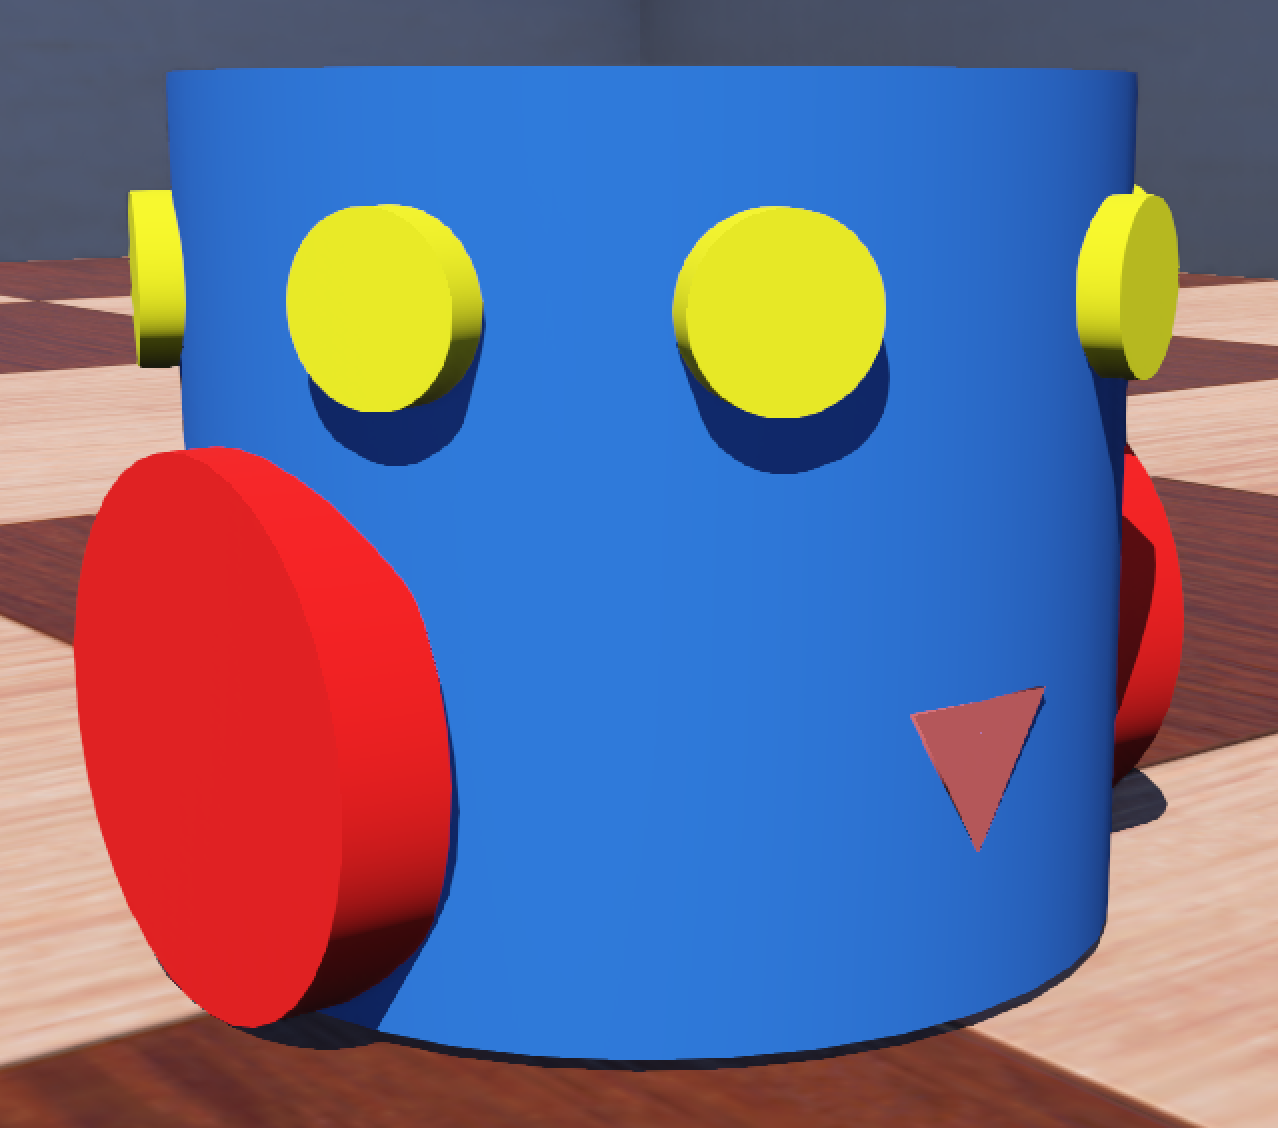
\includegraphics[width=\linewidth]{\images/chapter3/robot.png}
	\caption{Plain rendering}
  	\label{fig:ch-3:robot-1}
  \end{subfigure}
  \begin{subfigure}[b]{0.4\linewidth}
  	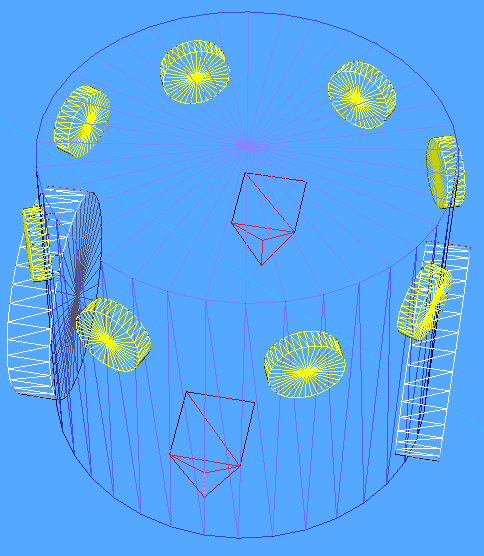
\includegraphics[width=\linewidth]{\images/chapter3/robot1.png}
	\caption{Wireframe rendering}
  	\label{fig:ch-3:robot-2}
  \end{subfigure}
  \caption{Custom robot view}
  \label{fig:ch-3:robot-view}
\end{figure}

The robot is positioned at the center of an arena of 1.5m x 2m surrounded by walls. This position is communicated to the robot and it becomes its initial state. In order to avoid obstacles while moving, a simple algorithm has been used that turns around the robot when the front sensors tell the presence of a solid object near 15 cm of distance.

\section{State Prediction}

Webots introduces the concept of supervisor which is a class forming part of the Webots API that simulates human actions in the environment. For instance, it can restart the simulation and put the robot in a random position or it can measure the trajectory of the robot at each step. Notice that this last concept is strictly restricted to the Webots simulator and it is not part of the command line of any real robot. Combined along with the compass sensor data will be useful to get the true robot state $\mathbf{x_t} = [x_t, y_t, \theta_t]^T$ where $x_t \text{ and } y_t$ are the coordinates of the robot translated to the GRF and $\theta_t$ is the orientation of the robot over the virtual north at time $t$. The predicted state will be $\mathbf{\hat{x}_{t}} = [\hat{x}_t, \hat{y}_t, \hat{\theta}_t]^T$ and it can be updated recursively based on the previous given state and thus at time $t+1$ the state will be $\mathbf{\hat{x}_{t+1}} = \mathbf{\hat{x}_{t}} + [\Delta x, \Delta y, \Delta \theta]^T$. This corresponds to the second line of the Bayes Filter algorithm (see algorithm \ref{ch-2:algo:bayes-filter}), that is, $\overline{bel}(\mathbf{x_t})$.

Cyberbotics' Robot Curriculum website\cite{webots-curri-odometry} provides a good explanation about how to implement odometry technique and which parameters need to be calibrated in order to have a precise implementation. These parameters need to be found experimentally since they are not measurable directly with enough precision: the distance of increment for the left wheel, the right wheel and the distance between both wheels. To have those values well configured four tests need to be performed:

\begin{itemize}
\item \textit{Increments per tour: } the number of motor increments made per one complete wheel rotation. While the robot have gone forward, the wheel had made one complete tour. 
\item \textit{Axis wheel ratio: } the diameter of the wheels divided by the distance between them. The robot turns around on its own axis and the goal is to end up at the same position that it began.
\item \textit{Wheels diameters: } the robot follows a square trajectory and it should end up at the same position where it started. If that is not the case, the diameter of one wheel can differ to the other as it is shown in figure \ref{fig:ch-3:wheel-diameters}.
\item \textit{Scaling factor: } it configures the scale of the trajectory.
\end{itemize}

\begin{figure}[h!]
  \centering
  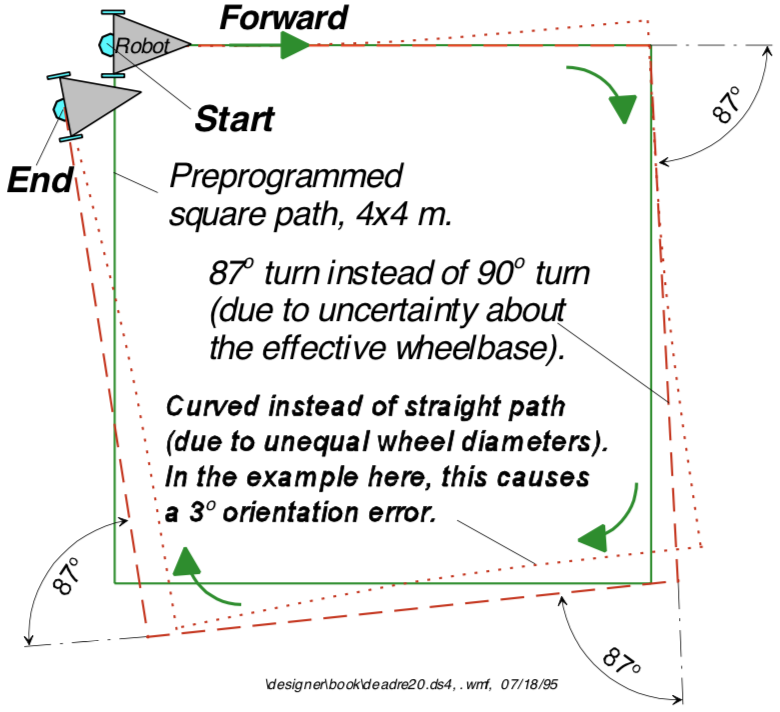
\includegraphics[width=0.6\linewidth]{\images/chapter3/wheel-diameters.png}
  \caption{Wheel diameters test.}
  \label{fig:ch-3:wheel-diameters}
  \source{Where am I?\cite{Feng:where-am-I}}
\end{figure}

After performing the tests and having an estimation of the corresponding values the results are shown in figure \ref{fig:ch-3:odometry-res}. The plots were taken in an aerial-view way where the axis represents the width and height of the arena and the lines mark the trajectory of the robot. On the one hand the blue line represents the true state pose of the robot obtained by the supervisor and compass data, on the other hand the orange line represents the predicted state pose of the robot using odometry techniques. The left-side image was obtained by running one simulation of the mobile robot with zero noise on its position sensors. Even though the odometry measurements approximate very well the true pose, they are still phased out due to the fact that the parameters used by odometry were found experimentally and thus some systematic error was introduced. The right-side image shows how the predicted robot state quickly starts to diverge from the true state due to noise associated with the position sensors that affects the data returned by the odometry technique. Thus as time goes the robot predicted state will be far from the true state; however, this problem should be resolved during the correction step in the Bayes Filter algorithm.

\begin{figure}[h!]
  \centering
  \begin{subfigure}[b]{0.47\linewidth}
  	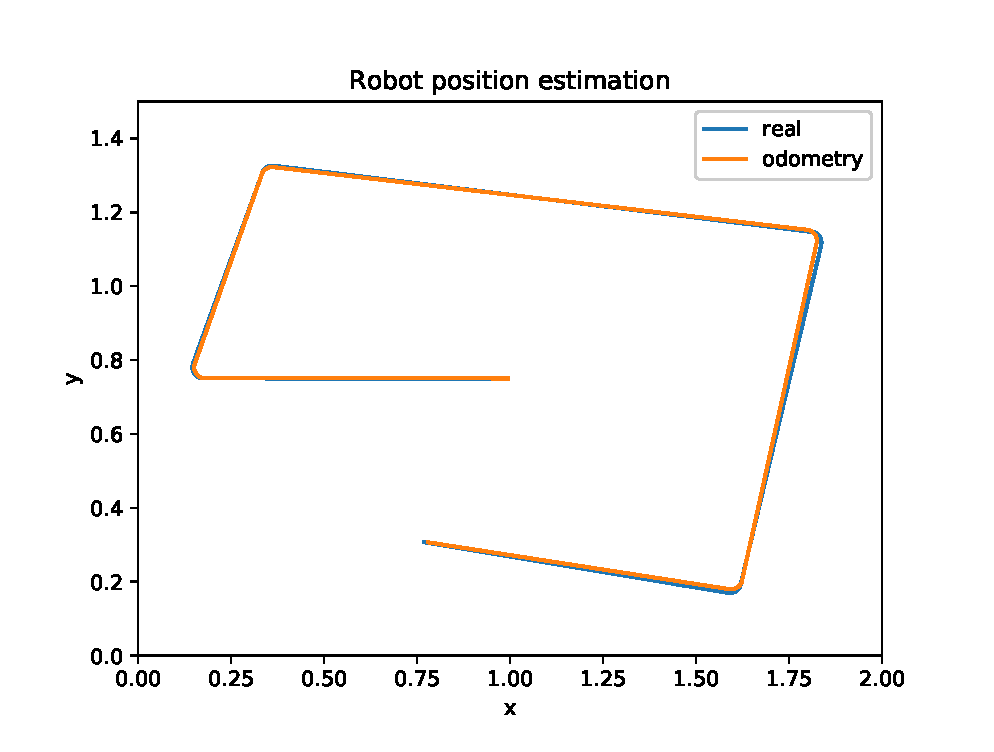
\includegraphics[width=\linewidth]{\images/chapter3/position-00-error.eps}
	\caption{Position Sensor Noise = 0}
  	\label{fig:ch-3:noise-0}
  \end{subfigure}
  \begin{subfigure}[b]{0.47\linewidth}
  	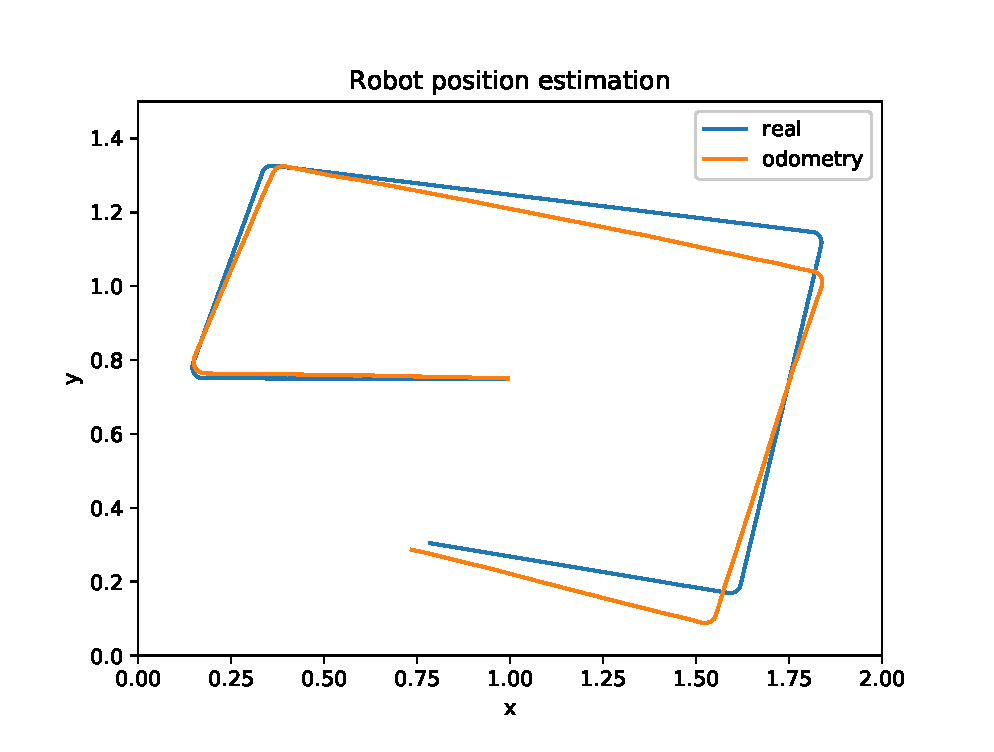
\includegraphics[width=\linewidth]{\images/chapter3/position-01-error.eps}
	\caption{Position Sensor Noise = 0.1}
  	\label{fig:ch-3:noise-1}
  \end{subfigure}
  \begin{subfigure}[b]{0.6\linewidth}
  	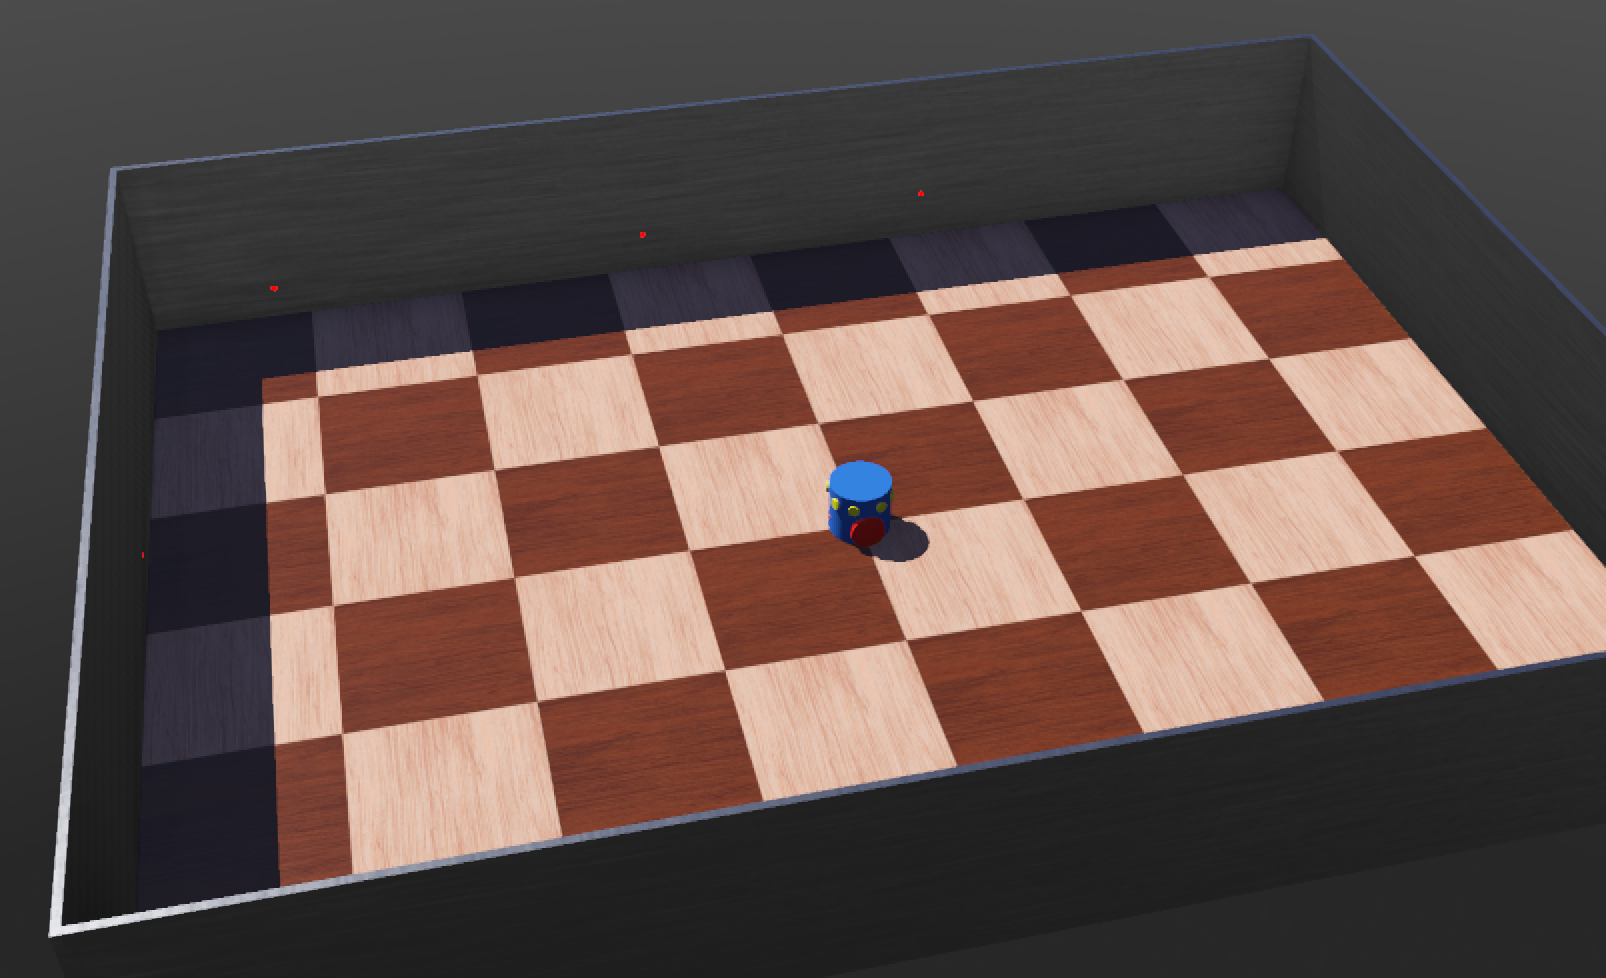
\includegraphics[width=\linewidth]{\images/chapter3/arena.png}
	\caption{Robot in the arena}
  	\label{fig:ch-3:arena}
  \end{subfigure}
  \caption{Odometry results}
  \label{fig:ch-3:odometry-res}
\end{figure}


\section{State Correction}

The second part of the Bayes Filter algorithm corresponds to the error correction state which implies calculating the current posterior distribution based on the previous posterior distribution which in practice corresponds to using the predicted state given by odometry and then using this data to calculate the probability of perceived the sensor measurements data in order to make the state correction. This corresponds to the third line of the Bayes Filter algorithm (see algorithm \ref{ch-2:algo:bayes-filter}), that is $bel(x_t)$.

There are two steps for performing the state correction. First, the robot-moving simulation runs for ten minutes in fast mode while collecting its distance sensor measurements along with true state pose data to train a model that can be capable of predicting distance sensor measurements given a certain state pose, that model will be represented by the function $\hat z(\mathbf{x_t})$. Second, given a predicted state $\mathbf{\hat x_t}$ provided by the odometry technique and sensor measurements $z_t$, a set of $m$ hypothesis regarding the true robot position is created using some variations of the given predicted state (described in more detail in section \ref{sec:ch-3:corr-odo-data}), that is, $\mathcal{X} = \{\mathbf{\hat x_t^1}, \mathbf{\hat x_t^2}, ..., \mathbf{\hat x_t^m}\}$. The hypothesis state which is closer to the true state, named best state and denoted as $\mathbf{\hat x_t^*}$,  will be chosen minimizing the function in equation \ref{eq:ch-3-optimization} and thus the odometry data will be corrected using this state value. Notice that this corresponds to searching the values of x that maximizes the conditional probability of distance sensor measurements given a state $x$ under the Bayes Filter approach.

\begin{equation}\label{eq:ch-3-optimization}
\mathbf{\hat x_t^*} =  \arg\min_\mathbf{x \in \mathcal{X}} (\hat z(\mathbf{x}) - z_t)^2 \approx \arg\max_x \eta \: p(z_t | x)
\end{equation}



\subsection{Collecting Pose and Sensor Data}

A data set is constructed using the \path{pandas} library where the features are the true robot state ($\mathbf{x_t}$) and the target variables are the sensor measurements ($\mathbf{z_t}$), the objective to do so is to generalize and predict sensor measurements given a certain robot state. 

\begin{table}[h]
\centering
    \begin{tabular}{lllllllllllll}
    \toprule
    \multicolumn{3}{c}{Features ($\mathbf{x_t}$)} & \multicolumn{8}{c}{Target ($\mathbf{z_t}$)} \\
    \cmidrule(r){1-3} \cmidrule(r){4-11}
    $x_t$ & $y_t$ & $\theta_t$ & $z_1$ & $z_2$ & $z_3$ & $z_4$ & $z_5$ & $z_6$ & $z_7$ & $z_8$ \\
    \midrule
    	    	0.98 & 0.75 & 179.99 & 1.02 & 0.76 & 0.76 & 1.04 & 1.04 & 0.76 & 0.76 & 1.02 \\
		0.91 & 0.74 & 180.00 & 0.95 & 0.76 & 0.76 & 1.12 &	1.12 & 0.76 & 0.76 & 0.95 \\
		0.72 &	0.74 &	180.00 &	0.74 &	 &	0.76 &	1.33 &	1.33 &	0.76 &	0.76 &	0.74\\
		1.03 &	1.04 &	208.22 &	0.99 &	0.67 &	0.40 &	 & 	0.92 &	1.19 &	1.00 &	1.30\\
		...\\
		0.29 &	0.58 &	212.58 &	0.25 &	0.31 &	0.88 &	1.06 &	1.68 &	0.98	&       0.54 &	0.47\\
    \bottomrule

    \end{tabular}
     \caption{Built Data Set}
     \label{tab:ch-3:built-data-set}
\end{table}

Table \ref{tab:ch-3:built-data-set} shows part of the collected data. Notice that some sensor measurements are missing intentionally. Once the simulation has run for ten minutes in fast mode the data set is saved into a csv file and then it was split in 80\% training and 20\% test. Then the \path{sklearn} library is used to create an ensemble of models employing the Random Forest technique with ten trees\footnote{Usually random forest works better with a bigger amount of trees but due to performance constrains only ten trees are used.}. The training data is used to train the ensemble of models and finally the accuracy is measured to be 99\%. This ensemble of models will be represented as a function $\hat z(\mathbf{x_t})$.

\subsection{Correcting Odometry Data}\label{sec:ch-3:corr-odo-data}
The algorithm for correcting the odometry data is divided in three parts. First, it takes a range of state values built on the predicted state $\mathbf{\hat x_t} = [\hat x_t, \hat y_t, \hat \theta_t]$, that is, $\mathcal{X} = \{\mathbf{\hat x_t^1}, \mathbf{\hat x_t^2}, ..., \mathbf{\hat x_t^m}\}$ these hypothesis are built based on all the possible state values near the predicted state defined by two parameters $\delta$ and $\omega$ for modifying the range of the $\hat x_t, \hat y_t$ coordinates and the range of the $\hat \theta_t$ angle respectively. The bigger these values, the higher the number of hypothesis to be evaluated. Second, it iterates over all hypothetic state values $\mathbf{x} \in \mathcal{X}$, and evaluates how probable is to be in state $ \mathbf{x} $ comparing the data provided by the distance sensors of the robot $z_t$, with the predicted distance sensor data provided by the function $\hat z(\mathbf{\cdot})$ previously obtained by training the model. Finally, it selects the best state value, that is, the hypothetic state value $\mathbf{\hat x_t^*} $ whose distance sensor prediction was more approximated to the real one using equation \ref{eq:ch-3-optimization}. The algorithm is illustrated below.

\IncMargin{1em}
\begin{algorithm}

\SetKwInOut{Input}{input}\SetKwInOut{Output}{output}
\Input{ $\hat x_t$, $\hat y_t$, $\hat \theta_t$, $\delta$, $\omega$, $z_t$, $\hat z(\mathbf{\cdot})$}
\Output{$\mathbf{\hat x_t^*} $}
\BlankLine
  $\mathcal{X} \leftarrow \emptyset$\\
  $Z \leftarrow \emptyset$\\
  $x_{range} \leftarrow [\hat x_t + \delta, \hat x_t - \delta]$\\
  $y_{range} \leftarrow [\hat y_t + \delta, \hat y_t - \delta]$\\
  $\theta_{range} \leftarrow [\hat \theta_t + \omega, \hat \theta_t - \omega]$\\
  \BlankLine
  \tcp{First part: creation of set $\mathcal{X}$ }
  \ForEach{$x \in x_{range}$ }{
  	\ForEach{$y \in y_{range}$} {
		\ForEach{$\theta \in \theta_{range}$} {
			$\mathcal{X}  \leftarrow \mathcal{X} \cup \lbrace \langle x, y, \theta \rangle \rbrace$
		}
	}
  }
  \BlankLine
  \tcp{Second part: calculate predictions}
  \ForEach{$\mathbf{x} \in \mathcal{X}$} {
  	$error \leftarrow (\hat z(\mathbf{x}) - z_t) ^ 2$\\
  	$\mathcal{E} \leftarrow \mathcal{E} \cup \{error\}$\\
  }
  \BlankLine
  \tcp{Third part: best state}
  $i \leftarrow \text{ get index of }min(\mathcal{E})$\\
  $\mathbf{\hat x_t^*} \leftarrow \mathcal{X}[i]$\\
  
  \Return $\mathbf{\hat x_t^*} $
\caption{Correction State Algorithm: Calculate Best State Value}

\label{algo:ch-3:x-creation}
\end{algorithm}\DecMargin{1em}

An implementation in Python can be found in appendix \ref{sec:ap:correction-state-algo}.

\section{Results}
The model for predicting distance sensor measurements is trained when the simulation starts and the algorithm to calculate the best state value is executed each 450 robot steps, that is, approximately one meter of robot traveled distance. Additionally, the distance sensors are configured to have a standard deviation of 0.01 using a lookup table as it is shown in section \ref{sec:ch-2:sensors} and the position sensors are configured to have a standard deviation of 0.1 using its noise attribute. The experiment runs with $\delta=10$ and $\omega=3$ and thus a square area of 20 cm around the predicted state is considered to make the correction step. Figure \ref{fig:ch-3:pose-correction} shows the results. The green points represent the best state value found, that means that the algorithm was called three times during the simulation and thus the predicted data is then corrected. 

\begin{figure}[h!]
  \centering
  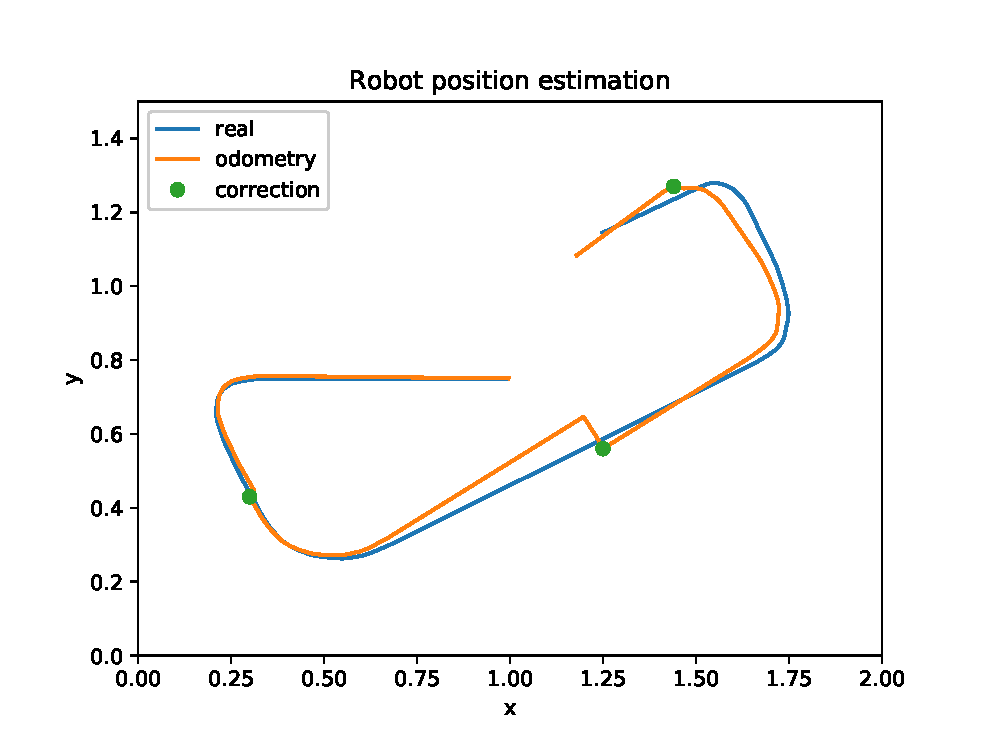
\includegraphics[width=0.7\linewidth]{\images/chapter3/position3.eps}
  \caption{Pose correction}
  \label{fig:ch-3:pose-correction}
\end{figure}

Notice that the number of hypothesis (the size of set $\mathcal{X}$) will be in this case $|x_{range}|\times|y_{range}|\times|\theta_{range}| = 20\times20\times3 = 1200$ and each hypothesis will be processed by the prediction function $\hat z(\mathbf{\cdot})$ which uses ten trees to take a decision and therefore this method is computationally heavy and thus, it requires high computational resources which is not usually the case for a simple robot. 

\section{Discussion and Further Work}

The Random Forest technique shows a very high accuracy on the test data caused by highly repeated data which means that the robot could have been passed by the same place multiple times while collecting data, making easy to predict a value already seen during training. Additionally, figure \ref{fig:ch-3:pose-correction} shows that the first two state corrections are very accurate but the third one is not. This can be caused because the data set used to train the model was obtained with only one run of the simulation and thus the predictions are not very accurate when the robot visits a place that was not previously visited during the collection data process. A solution to the two previously aforementioned problems would be to execute multiple simulations while collecting data initializing the robot position into a random place in the arena, and to add randomness behavior to the control actions when moving the robot in order to obtain a more generic dataset.

The algorithm has a poor performance when the number of hypothetic state values is high. A solution to this problem could be executing the Correction State algorithm more periodically, using smaller values for the $\delta$ and $\omega$ parameters. Additionally, some other prediction techniques could be more efficient than Random Forest and thus a comparison among them should be performed.

The size of the arena is ideal for running simulations but real-world scenarios can be less predictive and far more complex. Thus a more realistic environment will be created.






